%! Tex program = xelatex

\documentclass{article}
\usepackage[left=2cm, right=2cm, lines=45, top=0.8in, bottom=0.7in]{geometry}

% \usepackage[utf8]{inputenc} % 用于指定文件的编码格式  
% \usepackage[fontset=ubuntu]{ctex} % 使用ctex宏包并指定字体集

\usepackage{xeCJK}
\usepackage{setspace}
\usepackage[linesnumbered,ruled,vlined]{algorithm2e}
\usepackage[colorlinks,linkcolor=blue]{hyperref}%用于插入超链接
\onehalfspacing
\setmainfont{Times New Roman}
% \setCJKmainfont{Songti SC}
% \setCJKfamilyfont{song}{Songti SC}
\usepackage{color}
\usepackage{graphicx} % 导入图像的宏包、单图
\usepackage{subfigure} % 导入图像的宏包、子图
\usepackage{listings}
\lstset{breaklines}%这条命令可以让LaTeX自动将长的代码行换行排版
\lstset{extendedchars=false}%这一条命令可以解决代码跨页时,章节标题,页眉等汉字不显示的问题

\usepackage{tikz}

% 定义自定义颜色
\definecolor{textgray}{RGB}{82,82,82}
\definecolor{keywordorange}{RGB}{182,75,45}
\definecolor{operatorpurple}{RGB}{139,61,237}
\definecolor{codebg}{RGB}{248,248,248}
\definecolor{commentgray}{RGB}{121,121,121}
\definecolor{symbolgreen}{RGB}{47,100,70}  % 新增符号颜色



\lstdefinestyle{algorithm}{
    language=C++,
    keywordstyle=\color{keywordorange},    % 关键字颜色
    identifierstyle=\color{textgray},      % 标识符颜色
    basicstyle=\ttfamily\color{textgray},  % 基本文本颜色
    commentstyle=\color{commentgray}\textit,  % 注释颜色
    stringstyle=\color{keywordorange}\ttfamily,  % 字符串颜色
    showstringspaces=false,
    numbers=left,
    numberstyle=\small\color{textgray},    % 行号颜色
    backgroundcolor=\color{codebg},        % 背景颜色
    frame=none,                            % 移除边框
    breaklines=true,                       % 自动换行
    extendedchars=false,
    literate=
        {0}{{\textcolor{operatorpurple}{0}}}{1}
        {1}{{\textcolor{operatorpurple}{1}}}{1}
        {2}{{\textcolor{operatorpurple}{2}}}{1}
        {3}{{\textcolor{operatorpurple}{3}}}{1}
        {4}{{\textcolor{operatorpurple}{4}}}{1}
        {5}{{\textcolor{operatorpurple}{5}}}{1}
        {6}{{\textcolor{operatorpurple}{6}}}{1}
        {7}{{\textcolor{operatorpurple}{7}}}{1}
        {8}{{\textcolor{operatorpurple}{8}}}{1}
        {9}{{\textcolor{operatorpurple}{9}}}{1}
        {=}{{\textcolor{symbolgreen}{=}}}{1}
        {>}{{\textcolor{symbolgreen}{>}}}{1}
        {<}{{\textcolor{symbolgreen}{<}}}{1}
        {:}{{\textcolor{symbolgreen}{:}}}{1}
}


% 定义颜色
\definecolor{keywordblue1}{RGB}{79,113,190}    % 蓝色关键字
\definecolor{commentgray}{RGB}{127,127,127}   % 灰色注释
\definecolor{funcgreen}{RGB}{79,173,91}      % 绿色函数名
\definecolor{lightgreenbg}{RGB}{229,240,219}  % 浅绿色背景


\lstdefinestyle{algorithmPPT}{
    language=C++,
    keywordstyle=\color{keywordblue1},         % 关键字为蓝色
    commentstyle=\color{commentgray}\itshape, % 注释为灰色斜体
    basicstyle=\ttfamily\color{black},        % 基本文本为黑色
    backgroundcolor=\color{lightgreenbg},     % 背景为浅绿色
    frame=none,                               % 无边框
    breaklines=true,                          % 自动换行
    showstringspaces=false,
    numbers=left,                             % 显示行号
    numberstyle=\small\color{black},          % 行号样式
    numbersep=5pt,  
    % 自定义关键字
    morekeywords={foreach, do, then, else, if, while},  % 关键字
    % % 函数名颜色 - 使用更精确的匹配
    % moredelim=[b][\color{funcgreen}]{DFS},    % DFS函数
    % moredelim=[b][\color{funcgreen}]{BFS},    % BFS函数
    % 注释样式
    morecomment=[s][\color{commentgray}\itshape]{<}{>}
}


\begin{document}

\title{算法作业9}
\author{2207070213 赖立勋} % 替换成自己的学号和姓名
\maketitle

% 每道题包括题目问题描述和解答。答案请填下解答区。
\section{PPT补完计划}
\subsection{问题描述}

请证明:

1. 无向图的广度优先遍历中,不存在BE;

2. 无向图的广度优先遍历中,不存在DE。

\subsection{解答}

\subsubsection{1. 证明无向图BFS中不存在后向边(Back Edge)}

\noindent\textbf{证明:}\\
设存在后向边$(u,v)$,其中$v$是$u$的祖先节点。我们通过反证法证明这是不可能的。

\begin{enumerate}
    \item 若$v$是$u$的祖先,则在BFS中:
    \begin{itemize}
        \item $v.dis < u.dis$(BFS按层次遍历的性质)
        \item 具体地,$u.dis = v.dis + k$,其中$k \geq 2$(因为$v$是祖先而非父节点)
    \end{itemize}
    
    \item 然而,由于$(u,v)$是无向图中的边:
    \begin{itemize}
        \item 当$v$被发现时,$u$作为$v$的邻居节点应立即被发现
        \item 此时必有$u.dis = v.dis + 1$
    \end{itemize}
    
    \item 这与步骤1中$u.dis = v.dis + k$ $(k \geq 2)$矛盾
\end{enumerate}

\noindent 因此,无向图的BFS中不存在后向边。

\subsubsection{2. 证明无向图BFS中不存在前向边(Descendant Edge)}

\noindent\textbf{证明:}\\
设存在前向边$(u,v)$,其中$v$是$u$的后代但非子节点。同样使用反证法。

\begin{enumerate}
    \item 由于$v$是$u$的后代但非直接子节点:
    \begin{itemize}
        \item $v.dis \geq u.dis + 2$
        \item (因$v$至少要经过$u$的一个子节点才能到达)
    \end{itemize}
    
    \item 但在无向图中,由于$(u,v)$是一条边:
    \begin{itemize}
        \item 当$u$被BFS访问时(变为灰色)
        \item $v$作为$u$的邻居会被立即检查
        \item 若$v$为白色,会立即入队,且$v.dis = u.dis + 1$
        \item 若$v$已被发现,则$v.dis \leq u.dis + 1$
    \end{itemize}
    
    \item 这与步骤1中$v.dis \geq u.dis + 2$矛盾
\end{enumerate}

\noindent 因此,无向图的BFS中不存在前向边。
\subsection{参考答案}


\paragraph{1.利用反证法,假设其存在,然后推出矛盾即可。}

\href{https://github.com/Shannju/njucser_helphelp/blob/main/Algorithm%E7%AE%97%E6%B3%95/%E7%AD%94%E6%A1%88/P4~7.pdf}{2版 9.1题}

\begin{itemize}
    \item 假设在遍历$v$时发现了BE,指向了$w$,则在之前BFS中,队列弹出$w$,会发现$v$为$w$的为访问过的邻居,则BE其实是TE,矛盾。
    \item 假设在遍历$v$时发现了DE,指向了$w$,实际上还是TE,矛盾。
\end{itemize}


\paragraph{2.利用反证法,假设其存在,然后推出矛盾即可。}

\href{https://github.com/Shannju/njucser_helphelp/blob/main/Algorithm%E7%AE%97%E6%B3%95/%E7%AD%94%E6%A1%88/%E7%AE%97%E6%B3%95%E7%AD%94%E6%A1%88csdn%EF%BC%88%E5%8A%A9%E6%95%99%E5%B7%B2%E5%88%A0%E9%99%A4.pdf}{1版 5.1题}

\begin{enumerate}
    \item 假设存在BE:
    \begin{itemize}
        \item 若遍历到某白色节点v时,发现其黑色祖先邻居w
        \item 则说明w先于v被遍历到了,则w的所有邻居(包括v)已经被遍历过了
        \item v为2次遍历,矛盾,故vw是TE
        \item 因此不存在BE
    \end{itemize}
    
    \item 假设存在DE:
    \begin{itemize}
        \item 则遍历到某白色节点v时,发现一个DE:vw
        \item 则说明w是v的邻居,v一定先于其BFS树上的子节点先遍历w
        \item 故vw是TE,矛盾
        \item 因此不存在DE
    \end{itemize}
\end{enumerate}
%--------------------------------
% 每道题包括题目问题描述和解答。答案请填下解答区。

\pagebreak
\section{图解算法}
\subsection{问题描述}

对图9-1,设源点是3,请给出BFS之后,每个节点的parent和dis值。(默认采用数字序)

\begin{figure}[h]
    \centering
    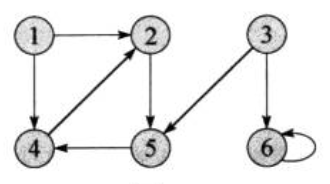
\includegraphics[width=0.5\linewidth]{Figure/9-1.png}
    \caption{图9-1}
    \label{fig:9-1 raw}
\end{figure}

对图9-2,设源点是u,请给出BFS之后,每个节点的parent和dis值。(默认采用字母序)

\begin{figure}[h]
    \centering
    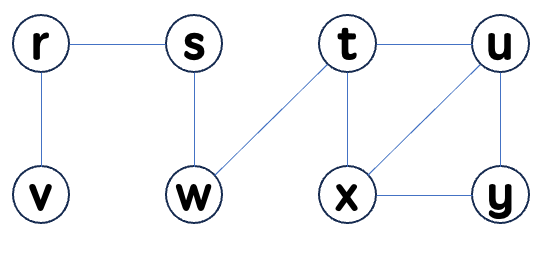
\includegraphics[width=0.5\linewidth]{Figure/9-2.png}
    \caption{图9-2}
    \label{fig:9-2 raw}
\end{figure}


\subsection{解答}

\subsubsection{对图9-1执行BFS并确定每个节点的parent和dis值}

\begin{figure}[htbp]
    \centering
    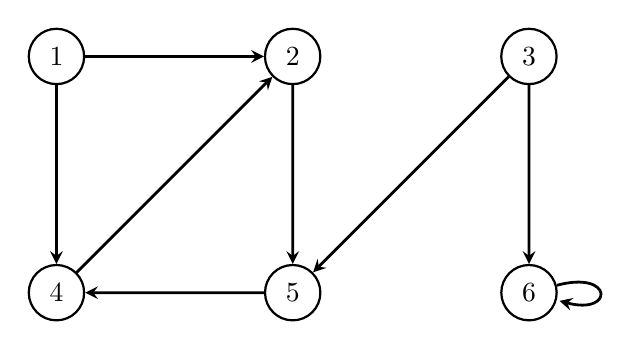
\begin{tikzpicture}[
        scale=1.5,                    % Scale up the entire diagram
        node distance=3cm,            % Increased spacing between nodes
        every node/.style={
            circle, 
            draw, 
            minimum size=2em,       % Slightly larger nodes
            inner sep=4pt             % More internal padding
        },
        >=stealth,
        thick,
        arrow/.style={->, line width=1pt}
    ]
        % 节点
        \node (1) {1};
        \node (4) [below of=1] {4};
        \node (2) [right of=1] {2};
        \node (5) [below of=2] {5};
        \node (3) [right of=2] {3};
        \node (6) [below of=3] {6};
        
        % 边
        \draw[arrow] (1) -- (2);
        \draw[arrow] (1) -- (4);
        \draw[arrow] (4) -- (2);
        \draw[arrow] (2) -- (5);
        \draw[arrow] (5) -- (4);
        \draw[arrow] (3) -- (5);
        \draw[arrow] (3) -- (6);
        \draw[arrow] (6) edge [loop right] (6);
    \end{tikzpicture}
    \caption{图9-1}
    \label{fig:9-1}
\end{figure}

\noindent\textbf{解答:}\\
给定源点为节点3,我们对图9-1执行广度优先搜索(BFS)。由于图是有向图,部分节点可能无法从源点到达。以下是每个节点在BFS完成后的parent和dis值:

\begin{center}
\begin{tabular}{|c|c|c|}
    \hline
    节点编号 & Parent & dis值 \\
    \hline
    1 & - & $\infty$ \\
    2 & 4 & 3 \\
    3 & - & 0 \\
    4 & 5 & 2 \\
    5 & 3 & 1 \\
    6 & 3 & 1 \\
    \hline
\end{tabular}
\end{center}

\noindent\textbf{详细步骤如下:}

\begin{enumerate}
    \item \textbf{初始化:}
    \begin{itemize}
        \item 标记所有节点为未访问(白色)。
        \item 设置源点3的`dis`值为0,`parent`为无(-)。
        \item 将节点3加入队列。
    \end{itemize}
    
    \item \textbf{第一层(dis = 0):}
    \begin{itemize}
        \item 访问节点3:
        \begin{itemize}
            \item 邻居节点为5和6。
            \item 设置节点5和6的`dis`值为1,`parent`均为3。
            \item 将节点5和6加入队列。
        \end{itemize}
    \end{itemize}
    
    \item \textbf{第二层(dis = 1):}
    \begin{itemize}
        \item 访问节点5:
        \begin{itemize}
            \item 邻居节点为4。
            \item 设置节点4的`dis`值为2,`parent`为5。
            \item 将节点4加入队列。
        \end{itemize}
        \item 访问节点6:
        \begin{itemize}
            \item 邻居节点为自身(已访问),无需操作。
        \end{itemize}
    \end{itemize}
    
    \item \textbf{第三层(dis = 2):}
    \begin{itemize}
        \item 访问节点4:
        \begin{itemize}
            \item 邻居节点为2。
            \item 设置节点2的`dis`值为3,`parent`为4。
            \item 将节点2加入队列。
        \end{itemize}
    \end{itemize}
    
    \item \textbf{第四层(dis = 3):}
    \begin{itemize}
        \item 访问节点2:
        \begin{itemize}
            \item 邻居节点为5(已访问),无需操作。
        \end{itemize}
    \end{itemize}
    
    \item \textbf{结束:}
    \begin{itemize}
        \item 队列为空,BFS结束。
    \end{itemize}
    
\end{enumerate}

\subsubsection{对图9-2执行BFS并确定每个节点的parent和dis值}


\begin{figure}[htbp]
    \centering
    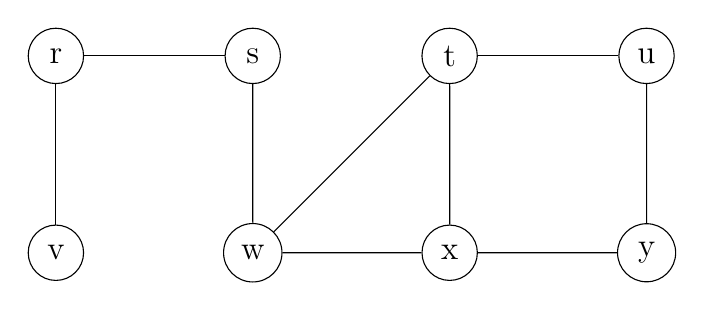
\begin{tikzpicture}[
        scale=1.5,
        node distance=2.5cm,
        every node/.style={
            circle, 
            draw, 
            minimum size=2em,
            inner sep=4pt,
            font=\large
        }
    ]
        % First component (r-s-v-w)
        \node (r) {r};
        \node (s) [right of=r] {s};
        \node (v) [below of=r] {v};
        \node (w) [below of=s] {w};
        
        % Second component (t-u-x-y)
        \node (t) [right of=s] {t};
        \node (u) [right of=t] {u};
        \node (x) [below of=t] {x};
        \node (y) [below of=u] {y};
        
        % Edges
        \draw (r) -- (s);
        \draw (r) -- (v);
        \draw (s) -- (w);
        \draw (t) -- (u);
        \draw (t) -- (x);
        \draw (u) -- (y);
        \draw (x) -- (y);
        \draw (w) -- (t);
        \draw (w) -- (x);
    \end{tikzpicture}
    \caption{图9-2}
    \label{fig:9-2}
\end{figure}

\noindent\textbf{解答:}\\
给定源点为节点u,我们对图9-2执行广度优先搜索(BFS)。以下是每个节点在BFS完成后的parent和dis值:

\begin{center}
\begin{tabular}{|c|c|c|}
    \hline
    节点 & Parent & dis值 \\
    \hline
    r & s & 4 \\
    s & w & 3 \\
    t & u & 1 \\
    u & - & 0 \\
    v & r & 5 \\
    w & t & 2 \\
    x & t & 2 \\
    y & u & 1 \\
    \hline
\end{tabular}
\end{center}

\noindent\textbf{详细步骤如下:}

\begin{enumerate}
    \item \textbf{初始化:}
    \begin{itemize}
        \item 标记所有节点为未访问(白色)
        \item 设置源点u的dis值为0,parent为无(-)
        \item 将节点u加入队列
    \end{itemize}
    
    \item \textbf{第一层(dis = 0):}
    \begin{itemize}
        \item 访问节点u,发现邻居t和y
        \item 设置t和y的dis值为1,parent为u
    \end{itemize}
    
    \item \textbf{第二层(dis = 1):}
    \begin{itemize}
        \item 访问t:发现w和x,设置它们的dis值为2,parent为t
        \item 访问y:邻居均已访问或在队列中
    \end{itemize}
    
    \item \textbf{第三层(dis = 2):}
    \begin{itemize}
        \item 访问w:发现s,设置其dis值为3,parent为w
        \item 访问x:邻居均已访问
    \end{itemize}
    
    \item \textbf{第四层(dis = 3):}
    \begin{itemize}
        \item 访问s:发现r,设置其dis值为4,parent为s
    \end{itemize}
    
    \item \textbf{第五层(dis = 4):}
    \begin{itemize}
        \item 访问r:发现v,设置其dis值为5,parent为r
    \end{itemize}
\end{enumerate}
%--------------------------------
% 每道题包括题目问题描述和解答。答案请填下解答区。
\section{有环图的检测}
\subsection{问题描述}

在PPT给出的DFS和BFS框架中,如何解决检测一个图是否存在环的问题?

\subsection{解答}

\subsubsection{PPT给出的DFS和BFS框架}

\paragraph{1.DFS}
\begin{lstlisting}[style=algorithmPPT]
    DFS(v)
        v.color:=GRAY
        <Preorder processing of node v>
        foreach neighbor w of v do
            if w.color = WHITE then
                <Exploratory processing of edge vw>
                DFS(w)
                <Backtrack processing of edge vw>
            else
                <Checking edge vw>
        <Postorder processing of node v>
        v.color:=BLACK
    \end{lstlisting}

\paragraph{2.BFS}
\begin{lstlisting}[style=algorithmPPT]
    BFS-WARRER(G)
    foreach node v in G do
        v.color:=WHITE; 
        v.parent=NULL 
        v.dis:=+∞;
    foreach node v in G do
        if v.color == WHITE then
            BFS(v)
\end{lstlisting}

\begin{lstlisting}[style=algorithmPPT]
            BFS(G)
                Initialize an empty queue queNode;
                v.color:=GRAY;
                v.dis:=0;
                queNode.EUQUE(v);
                while queNode != empty do
                    w:=queNode.DEQUE();
                    foreach neighbor x of w do
                        if x.color==WHITE then
                            x.color:=GRAY;
                            x.parent:=w;
                            x.dis:=w.dis+1;
                            queNode.ENQUEUE(x);
                        <processing of node w>;
                        w.color:=BLACK;
\end{lstlisting}

\subsubsection{框架中检测环的方法}

\paragraph{1.DFS\\}
\textbf{有向图:\\}

\begin{lstlisting}[style=algorithmPPT]
    DFS(v)
        v.color:=GRAY
        <Preorder processing of node v>
        foreach neighbor w of v do
            if w.color = WHITE then
                <Exploratory processing of edge vw>
                DFS(w)
                <Backtrack processing of edge vw>              
            else
                <Checking edge vw>
        \end{lstlisting}  

\begin{lstlisting}[style=algorithm]
                if w.color == GRAY then
                    // 发现后向边,存在环
                    return true
            \end{lstlisting}

\begin{lstlisting}[style=algorithmPPT]
        <Postorder processing of node v>
        v.color:=BLACK
    \end{lstlisting}

\textbf{无向图:\\}
\begin{lstlisting}[style=algorithmPPT]
    DFS(v)
        v.color:=GRAY
        <Preorder processing of node v>
        foreach neighbor w of v do
            if w.color = WHITE then
                <Exploratory processing of edge vw>
                DFS(w)
                <Backtrack processing of edge vw>              
            else
                <Checking edge vw>
        \end{lstlisting}  

\begin{lstlisting}[style=algorithm]
                if(w != parent) then
                    // 发现一个不是父节点的已访问节点,存在环
                    return true
            \end{lstlisting}

\begin{lstlisting}[style=algorithmPPT]
        <Postorder processing of node v>
        v.color:=BLACK
    \end{lstlisting}


\paragraph{2.BFS\\}
\textbf{有向图:\\}
\begin{lstlisting}[style=algorithmPPT]
    BFS-WARRER(G)
    foreach node v in G do
        v.color:=WHITE; 
        v.parent=NULL 
        v.dis:=+∞;
    foreach node v in G do
        if v.color == WHITE then
            BFS(v)
\end{lstlisting}

\begin{lstlisting}[style=algorithmPPT]
            BFS(G)
                Initialize an empty queue queNode;
                v.color:=GRAY;
                v.dis:=0;
                queNode.EUQUE(v);
                while queNode != empty do
                    w:=queNode.DEQUE();
                    foreach neighbor x of w do
                        if x.color==WHITE then
                            x.color:=GRAY;
                            x.parent:=w;
                            x.dis:=w.dis+1;
                            queNode.ENQUEUE(x);
                        <processing of node w>;
\end{lstlisting}
\begin{lstlisting}[style=algorithm]
                        else if x.color == GRAY and x != w.parent then
                            // 发现环
                            return true;
\end{lstlisting}
\begin{lstlisting}[style=algorithmPPT]
                        w.color:=BLACK;
\end{lstlisting}

\textbf{无向图:\\}
\begin{lstlisting}[style=algorithmPPT]
    BFS-WARRER(G)
    foreach node v in G do
        v.color:=WHITE; 
        v.parent=NULL 
        v.dis:=+∞;
    foreach node v in G do
        if v.color == WHITE then
            BFS(v)
\end{lstlisting}

\begin{lstlisting}[style=algorithmPPT]
            BFS(G)
                Initialize an empty queue queNode;
                v.color:=GRAY;
                v.dis:=0;
                queNode.EUQUE(v);
                while queNode != empty do
                    w:=queNode.DEQUE();
                    foreach neighbor x of w do
                        if x.color==WHITE then
                            x.color:=GRAY;
                            x.parent:=w;
                            x.dis:=w.dis+1;
                            queNode.ENQUEUE(x);
                        <processing of node w>;
                    \end{lstlisting}

\begin{lstlisting}[style=algorithm]
                        else if x != w.parent then
                            // 发现交叉边,存在环
                            return true
                        \end{lstlisting}

\begin{lstlisting}[style=algorithmPPT]
                        w.color:=BLACK;
\end{lstlisting}

\subsection{参考答案}

\paragraph{1.}

\href{https://github.com/Shannju/njucser_helphelp/blob/main/Algorithm%E7%AE%97%E6%B3%95/%E7%AD%94%E6%A1%88/P4~7.pdf}{2版 9.4题}

\noindent\textbf{检测环的方法:}

\begin{enumerate}
    \item \textbf{使用DFS检测:}
    \begin{itemize}
        \item 适用于有向图和无向图
        \item 当遇到灰色(正在访问中的)节点时,说明存在BE,即存在环
    \end{itemize}

    \item \textbf{使用BFS检测:}
    \begin{itemize}
        \item \underline{有向图:}
        \begin{itemize}
            \item 需要检测是否存在BE(指向黑色祖先的边)
            \item 注意:指向黑色节点的边不一定是BE,也可能是CE
            \item 需要额外判断两个节点是否有共同的parent来区分BE和CE
        \end{itemize}
        \item \underline{无向图:}
        \begin{itemize}
            \item 当遇到灰色节点时,表示存在CE(交叉边)
            \item 存在CE即表示存在环
        \end{itemize}
    \end{itemize}
\end{enumerate}

\paragraph{2.}

\href{https://github.com/Shannju/njucser_helphelp/blob/main/Algorithm%E7%AE%97%E6%B3%95/%E7%AD%94%E6%A1%88/%E7%AE%97%E6%B3%95%E7%AD%94%E6%A1%88csdn%EF%BC%88%E5%8A%A9%E6%95%99%E5%B7%B2%E5%88%A0%E9%99%A4.pdf}{1版 5.8题 改}

\noindent 解析:在遍历中,环的存在性,在有向图的DFS和BFS,或者无向图的DFS中等价于BE的存在性,而无向图的BFS不存在BE,因此等价于CE的存在性

\noindent\textbf{1)DFS的算法如下:}

\begin{lstlisting}[style=algorithm]
// to find if G has a circle with DFS
Algorithm: IF_CIRCLE_DFS(G)
    foreach node x in G do  //initialize visit
        x.visit := false
    has := false
    foreach node v in G do
        if v.visit = false then
            if G is a DG then  // G is a directed graph
                has := DFS_DG(v)
            else  // G is an undirected graph
                has := DFS_UG(v,-1)
            if has := true then
                return true
    return false

// DFS to find if there's a circle with node v in DG
Algorithm: DFS_DG(v)
    v.visit := true
    has := false
    foreach neighbor w of v do
        if w.visit = false then
            has := DFS_DG(w)
            if has := true then
                return true
        else
            return true
    return false

// DFS to find if there's a circle with node v in UG
Algorithm: DFS_UG(v,parent)
    v.visit := true
    has := false
    foreach neighbor w of v do
        if w.visit = false then
            has := DFS_UG(w,v)
            if has := true then
                return true
        else if w != parent then
            return true
    return false
\end{lstlisting}

\noindent\textbf{BFS的算法如下:}

\begin{lstlisting}[style=algorithm]
// to find if G has a circle with BFS
Algorithm: IF_CIRCLE_BFS(G)
    foreach node x in G do  //initialize visit
        x.visit := false
    has := false
    foreach node v in G do
        if v.visit = false then
            if G is a DG then  // G is a directed graph
                has := BFS_DG(v)
            else  // G is an undirected graph
                v.parent := -1
                has := BFS_UG(v)
            if has := true then
                return true
    return false

// BFS to find if there's a circle with node v in DG
Algorithm: BFS_DG(v)
    v.visit := true
    queNode.ENQUE(v)
    while queNode is not empty do
        w := queNode.DEQUE()
        foreach neighbor u of w do
            if u.visit = false then
                queNode.ENQUE(u)
            else
                return true
        w.visit := true
    return false

// BFS to find if there's a circle with node v in UG
Algorithm: BFS_UG(v)
    v.visit := true
    queNode.ENQUE(v)
    while queNode is not empty do
        w := queNode.DEQUE()
        foreach neighbor u of w do
            if u.visit = false then
                u.parent := w
                queNode.ENQUE(u)
            else if u != w.parent then
                return true
        w.visit := true
    return false
\end{lstlisting}
%--------------------------------
% 每道题包括题目问题描述和解答。答案请填下解答区。
\section{DFS与BFS生成树}
\subsection{问题描述}

给定一个连通图$G=<V,E>$,和一个顶点$u\in V$。假设已经找到了一棵以$u$为根节点的DFS树$T$,又找到了一棵以$u$为根节点的BFS树$T'$,满足$T=T'$。

1. 如果$G$是一个无向图,请证明$G=T$(也就是说,图的所有边都是TE);

2. 如果$G$是一个有向图,整个结论是否还成立?

\subsection{解答}

\noindent\textbf{解析:}\\
通过分析有向图和无向图在DFS和BFS中可能出现的边的类型,我们可以得出结论。

\noindent\textbf{1. 无向图的情况(证明$G=T$)}
\begin{itemize}
    \item 对于无向图$G$:
    \begin{itemize}
        \item DFS中只可能存在TE和BE
        \item BFS中只可能存在TE和CE
    \end{itemize}
    
    \item 若$G$在DFS中存在BE:
    \begin{itemize}
        \item 该BE边在同根节点的BFS中一定会被作为TE边
        \item 这将导致DFS树不等于BFS树
    \end{itemize}
    
    \item 因此:
    \begin{itemize}
        \item $G$在DFS中不能存在BE
        \item $G$只能包含TE
        \item 所以$G = T$
    \end{itemize}
\end{itemize}

\noindent\textbf{2. 有向图的情况(结论不成立)}
\begin{itemize}
    \item 对于有向图$G$:
    \begin{itemize}
        \item DFS中四种类型边(TE、BE、FE、CE)均可能存在
        \item BFS中除了DE外的边(TE、BE、CE)都可能存在
    \end{itemize}
    
    \item 若$G$在DFS中存在BE或CE:
    \begin{itemize}
        \item 在BFS中同样会存在BE和CE
        \item 这种情况下$G \neq T$
    \end{itemize}
    
    \item 因此结论在有向图中不成立
\end{itemize}

\subsection{参考答案}

\paragraph{1.}
\href{https://github.com/Shannju/njucser_helphelp/blob/main/Algorithm%E7%AE%97%E6%B3%95/%E7%AD%94%E6%A1%88/P4~7.pdf}{2版 9.7题 暂无答案,哪位大佬有答案给兄弟们分享一下}

\paragraph{2.}
\href{https://github.com/Shannju/njucser_helphelp/blob/main/Algorithm%E7%AE%97%E6%B3%95/%E7%AD%94%E6%A1%88/%E7%AE%97%E6%B3%95%E7%AD%94%E6%A1%88csdn%EF%BC%88%E5%8A%A9%E6%95%99%E5%B7%B2%E5%88%A0%E9%99%A4.pdf}{1版 5.7题}
\noindent\textbf{解析:\\}抓住有向图和无向图在DFS和BFS中,边可能的各种类型进行分析即可;

\noindent\textbf{解答如下:}

\noindent 1)证明:对于无向图G而言,DFS只可能存在TE和BE,BFS只可能存在TE和CE,而如果G在DFS中存在BE,则在同根节点的BFS时,该BE边一定会被作为BFS树的TE边,从而DFS树不可能等于BFS树,因此,G在DFS时不存在BE,即只含TE,G = T,得证;

\noindent 2)结论不成立。因为对于有向图G而言,DFS四种类型边均可能存在,BFS除了DE之外都可能存在,因此只要G在DFS中存在BE或者CE,则在BFS中同样存在BE和CE,故此时G≠T,因此结论不成立;反例略;
\end{document}
